% Deterministic vector renderer for paper/figures/fig-scenario.pdf.
% The requested delivery path figures/fig-scenario.pdf is a byte-identical copy.
% The editable diagrams.net source is paper/figures/fig-scenario.drawio.
% Compile from the repository root with:
%   pdflatex -interaction=nonstopmode -halt-on-error -file-line-error \
%     -output-directory=paper/figures -jobname=fig-scenario \
%     paper/figures/fig-scenario-render.tex
\documentclass[tikz,border=0pt]{standalone}
\usepackage[T1]{fontenc}
\usepackage[condensed,sfdefault,type1]{roboto}
\usepackage{pifont}
\usetikzlibrary{arrows.meta,calc,decorations.pathreplacing}

\pdfinfo{
  /Title (Authenticated but unauthorized)
  /Subject (5D H-NGAC authorization scenario)
}

\definecolor{permitfill}{HTML}{A6D6A6}
\definecolor{permitstroke}{HTML}{4A7A4A}
\definecolor{denyfill}{HTML}{F2C4C0}
\definecolor{denystroke}{HTML}{A03030}
\definecolor{transportfill}{HTML}{F7F5F3}
\definecolor{softgray}{HTML}{EEEEEE}
\definecolor{midgray}{HTML}{777777}
\definecolor{ink}{HTML}{202020}

\newcommand{\bodyfont}{\fontsize{7}{6.45}\selectfont}
\newcommand{\headfont}{\fontsize{7.6}{7.6}\selectfont\bfseries}

\begin{document}
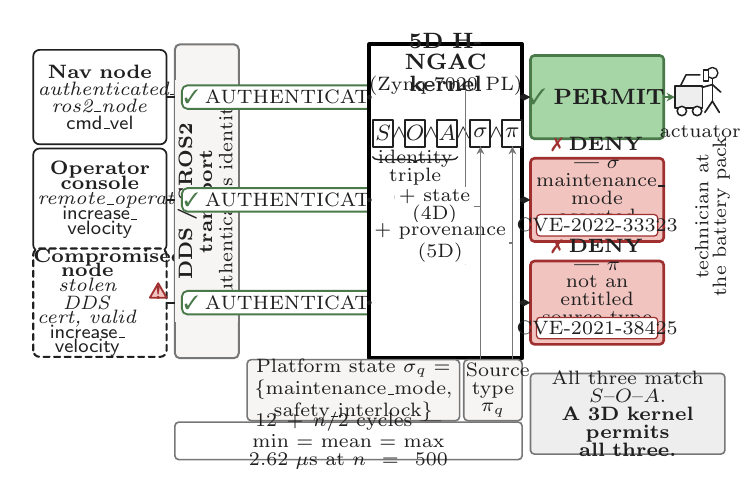
\begin{tikzpicture}[
  x=1bp,
  y=1bp,
  line cap=round,
  line join=round,
  every node/.style={font=\bodyfont,text=ink,inner sep=0.8pt},
  flow/.style={draw=ink,line width=0.62pt,-{Stealth[length=3.0pt,width=3.1pt]}},
  inputflow/.style={draw=midgray,line width=0.55pt,-{Stealth[length=2.8pt,width=2.8pt]}},
  sender/.style={draw=ink,fill=white,line width=0.62pt,rounded corners=2.3pt},
  tag/.style={draw=denystroke,fill=white,line width=0.45pt,rounded corners=1.2pt}
]
  % Exact IEEE single-column width. The height is 2.167 in so every label
  % remains at or above 7 pt; a 1050:560 canvas cannot hold this copy at 7 pt.
  \path[use as bounding box] (0,0) rectangle (252,156);
  \fill[white] (0,0) rectangle (252,156);

  % Column 1: senders.
  \draw[sender] (2,114) rectangle (50,148);
  \node[align=center,text width=45pt] at (26,131) {%
    \textbf{Nav node}\\[-0.3pt]
    \textit{authenticated\_}\\[-0.3pt]
    \textit{ros2\_node}\\[-0.3pt]
    \textsf{cmd\_vel}};

  \draw[sender] (2,75.5) rectangle (50,112.5);
  \node[align=center,text width=45pt] at (26,94) {%
    \textbf{Operator}\\[-1.0pt]
    \textbf{console}\\[-1.0pt]
    \textit{remote\_operator}\\[-1.0pt]
    \textsf{increase\_}\\[-1.0pt]
    \textsf{velocity}};

  \draw[draw=ink,fill=white,line width=0.75pt,dash pattern=on 2.2pt off 1.6pt,
        rounded corners=2.3pt]
    (2,37.5) rectangle (50,76.5);
  \node[align=center,text width=39pt] at (21.5,57) {%
    \textbf{Compromised}\\[-1.2pt]
    \textbf{node}\\[-1.2pt]
    \textit{stolen DDS}\\[-1.2pt]
    \textit{cert, valid}\\[-1.2pt]
    \textsf{increase\_}\\[-1.2pt]
    \textsf{velocity}};
  \path[draw=denystroke,fill=denyfill,line width=0.65pt]
    (47.0,64.0) -- (50.0,58.8) -- (44.0,58.8) -- cycle;
  \node[font=\fontsize{7}{7}\selectfont\bfseries,text=denystroke]
    at (47.0,60.7) {!};

  % Column 2: one neutral transport box spanning all request rows.
  \draw[draw=midgray,fill=transportfill,line width=0.72pt,rounded corners=1.8pt]
    (53,37) rectangle (76,150);

  % The three request streams use identical geometry and neutral ink.
  \draw[flow] (50,131) -- (123,131);
  \draw[flow] (50,94) -- (123,94);
  \draw[flow] (50,57) -- (123,57);

  \node[rotate=90,fill=transportfill,align=center,text width=86pt,
        font=\fontsize{7.2}{7.3}\selectfont]
    at (64.5,93.5) {\textbf{DDS / SROS2 transport}\\authenticates identity};

  % Three exact clones: transport identity authentication is deliberately equal.
  \foreach \yy in {131,94,57}{
    \node[draw=permitstroke,fill=white,line width=0.68pt,rounded corners=2pt,
          minimum width=40.5pt,minimum height=8.5pt,align=center]
      at (95.5,\yy) {\textcolor{permitstroke}{\ding{51}}\;AUTHENTICATED};
  }

  % Column 3: the 5D decision primitive.
  \draw[draw=black,fill=white,line width=1.45pt] (123,37) rectangle (178,150);
  \node[font=\headfont,align=center,text width=51pt] at (150.5,143.5) {5D H-NGAC kernel};
  \node[align=center] at (150.5,135.2) {(Zynq-7020 PL)};

  % Row ports make the correspondence with all three outcomes explicit.
  \foreach \yy in {131,94,57}{
    \fill[ink] (123,\yy) circle (0.85pt);
    \fill[ink] (178,\yy) circle (0.85pt);
  }

  % Five square gates with AND conjunctions.
  \foreach \xx/\lab in {128/$S$,139.5/$O$,151/$A$,163/$\sigma$,174.5/$\pi$}{
    \draw[draw=ink,fill=white,line width=0.72pt] (\xx-3.6,113.2) rectangle (\xx+3.6,122.8);
    \node[font=\fontsize{7.8}{7.8}\selectfont\bfseries] at (\xx,118) {\lab};
  }
  \foreach \xx in {133.7,145.2,156.8,168.7}{
    \node[font=\fontsize{7.3}{7.3}\selectfont] at (\xx,118) {$\wedge$};
  }
  \draw[draw=midgray,line width=0.45pt] (157.6,71) -- (157.6,133);

  \draw[decorate,decoration={brace,mirror,amplitude=2.0pt},draw=ink,line width=0.5pt]
    (124.2,109.5) -- (154.8,109.5);
  \node[align=center,text width=31pt] at (139.5,101.6) {identity triple\\(3D)};
  \draw[draw=midgray,line width=0.45pt] (163,113.2) -- (163,91.5) -- (158.5,91.5);
  \node[fill=white,align=center,text width=27pt] at (146.5,91.5)
    {$+$ state\\(4D)};
  \draw[draw=midgray,line width=0.45pt] (174.5,113.2) -- (174.5,78.5) -- (172.5,78.5);
  \node[fill=white,align=center,text width=48pt] at (148.5,78.5)
    {$+$ provenance\\(5D)};

  % Inputs are request context, routed upward into the sigma and pi gates.
  \draw[draw=midgray,fill=transportfill,line width=0.58pt,rounded corners=1.5pt]
    (79,14.5) rectangle (155.5,36.5);
  \node[align=center,text width=72.5pt] at (117.25,25.5) {Platform state $\sigma_q =$\\
    \{maintenance\_mode,\\safety\_interlock\}};
  \draw[draw=midgray,fill=transportfill,line width=0.58pt,rounded corners=1.5pt]
    (157,14.5) rectangle (178,36.5);
  \node[align=center,text width=19.5pt] at (167.5,25.5) {Source\\type $\pi_q$};
  \draw[inputflow] (152.5,36.5) -| (163,113.2);
  \draw[inputflow] (167.5,36.5) -| (174.5,113.2);

  % Column 4: outcomes. Word, glyph, fill, and stroke redundantly encode result.
  \draw[draw=permitstroke,fill=permitfill,line width=0.95pt,rounded corners=1.5pt]
    (181,116) rectangle (229,146);
  \node[font=\fontsize{8}{8}\selectfont\bfseries] at (205,131)
    {\textcolor{permitstroke}{\ding{51}}\;PERMIT};

  \draw[draw=denystroke,fill=denyfill,line width=0.95pt,rounded corners=1.5pt]
    (181,79) rectangle (229,109);
  \node[align=center,text width=44pt] at (205,101.2)
    {\textcolor{denystroke}{\ding{55}}\;\textbf{DENY --- $\sigma$}\\maintenance\_\\mode asserted};
  \draw[tag] (183.2,81.0) rectangle (226.8,88.7);
  \node at (205,84.9) {CVE-2022-33323};

  \draw[draw=denystroke,fill=denyfill,line width=0.95pt,rounded corners=1.5pt]
    (181,42) rectangle (229,72);
  \node[align=center,text width=44pt] at (205,64.0)
    {\textcolor{denystroke}{\ding{55}}\;\textbf{DENY --- $\pi$}\\not an entitled source type};
  \draw[tag] (183.2,44.0) rectangle (226.8,51.7);
  \node at (205,47.9) {CVE-2021-38425};

  \draw[flow] (178,131) -- (181,131);
  \draw[flow] (178,94) -- (181,94);
  \draw[flow] (178,57) -- (181,57);

  % Right edge: only PERMIT reaches the actuator. The technician remains exposed.
  \draw[draw=permitstroke,line width=0.9pt,-{Stealth[length=3.0pt,width=3.1pt]}]
    (229,131) -- (233,131);
  % Rover / actuator icon.
  \draw[draw=ink,fill=softgray,line width=0.55pt] (233,127) rectangle (243,135);
  \draw[draw=ink,line width=0.55pt] (235,135) -- (237,139) -- (242,139);
  \draw[draw=ink,fill=white,line width=0.55pt] (235.5,126) circle (1.7pt);
  \draw[draw=ink,fill=white,line width=0.55pt] (241,126) circle (1.7pt);
  \draw[draw=ink,fill=white,line width=0.5pt] (246.5,139.7) circle (2.0pt);
  \draw[draw=ink,line width=0.6pt] (246.5,137.5) -- (246.5,129.5);
  \draw[draw=ink,line width=0.6pt] (242.8,134.5) -- (246.5,135.5) -- (249.5,132.8);
  \draw[draw=ink,line width=0.6pt] (246.5,129.5) -- (243.8,125.5);
  \draw[draw=ink,line width=0.6pt] (246.5,129.5) -- (249.0,125.5);
  \draw[draw=ink,fill=white,line width=0.5pt] (243.2,136.8) rectangle (245.2,140.8);
  \node[align=center,text width=24pt] at (239.5,118.5) {actuator};
  \node[rotate=90,align=center,text width=66pt] at (246.5,88)
    {technician at the battery pack};

  % Bottom callouts.
  \draw[draw=midgray,fill=white,line width=0.58pt,rounded corners=1.4pt]
    (53,0.5) rectangle (178,14);
  \node[align=center,text width=121pt] at (115.5,7.25)
    {$12+n/2$ cycles --- min = mean = max\\2.62 $\mu$s at $n=500$};

  \draw[draw=midgray,fill=softgray,line width=0.58pt,rounded corners=1.4pt]
    (181,2.5) rectangle (251,31.5);
  \node[align=center,text width=66pt] at (216,17)
    {All three match\\$S$--$O$--$A$.\\\textbf{A 3D kernel}\\\textbf{permits all three.}};
\end{tikzpicture}
\end{document}
